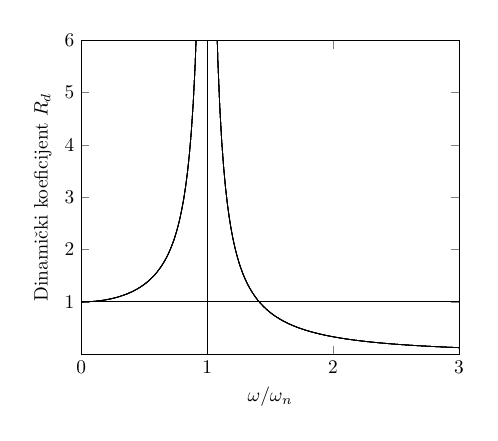
\begin{tikzpicture}[scale=0.7]
    \begin{axis} [
        ylabel = Dinamički koeficijent $R_d$,
        xlabel = $\omega/\omega_n$,
        xmin = 0, xmax = 3,
        ymin = 0, ymax = 6,
        xtick = {0, 1, 2, 3},
        ytick = {1, 2, 3, 4, 5, 6},
     ]

        \draw[thin] (1,0) -- (1,6);
        \draw[thin] (0,1) -- (3,1);
    \foreach \i in {1, 0.7, 0.4, 0.2, 0.1}
        {
            \addplot [
                domain=0:3,
                samples=200,
                color=black,
                thin,
            ]{1/abs(1-x^2)};
        }
    \end{axis}
\end{tikzpicture}
